\chapter{Extensibility and Multi-Tenancy}

Since the end of Dennard scaling, disaggregation has become the norm in
the datacenter.
%
Applications are typically broken into a compute and
storage tier separated by a high speed network, allowing each tier to be
provisioned, managed, and scaled independently.
%
However, this approach
is beginning to reach its limits.
%
Applications have evolved to become more data intensive than ever.
%
In addition to good performance, they often require rich and complex
data models such as social graphs, decision trees,
vectors~\cite{fb-memcache,parameter-server} etc.
%
Storage systems, on the other hand, have become faster with the help of
kernel-bypass~\cite{ramcloud,farm-txns}, but at the cost of their
interface – typically simple point lookups and updates.
%
As a result of using these simple interfaces to implement their data
model, applications end up stalling on network round-trips to the
storage tier.
%
Since the actual lookup or update takes only a few
microseconds at the storage server, these round-trips create a major
bottleneck, hurting performance and utilization.
%
Therefore, to fully
leverage these fast storage systems, applications will have to reduce
round-trips by pushing compute to them.

\begin{figure}[t]
\centering
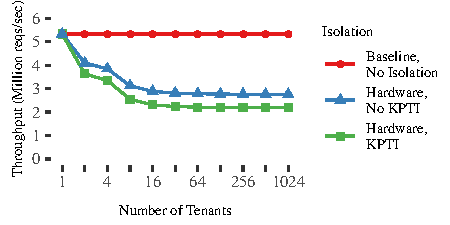
\includegraphics[width=1.0\columnwidth]{graphs/simulator.pdf}
\caption{Simulated throughput versus the number of tenants. With
	hardware isolation, even modestly increasing the number of
  tenants to 16 (just twice the number
	of cores) leads to a significant drop in throughput.
  ``No isolation'' represents an upper bound where isolation costs are zero.}
\label{fig:simulator}
\end{figure}


Pushing compute to these fast storage systems is
not straightforward.
%
To maximize utilization, these
systems need to be shared by multiple tenants,
but the cost for isolating tenants using conventional techniques is too
high.
%
Hardware isolation
requires a context switch that takes approximately
1.5 microseconds on a modern processor~\cite{splinter}.
%
This
is roughly equal to the amount of time it takes to
fully process an RPC at the storage server, meaning
that conventional isolation can hurt throughput by
a factor of 2 (Fig~\ref{fig:context-switches}).
%
Splinter relies on a type- and memory-safe language for isolation.
%
Tenants push
extensions – a tree traversal for example – written in the Rust
programming language~\cite{rust} to the system at runtime.
%
Splinter installs
these extensions.
%
Once installed, an extension can
be remotely invoked (executed) by the tenant in a
single round-trip.
%
For applications such as tree traversals which would ordinarily require
round-trips logarithmic in the size of the tree, splinter can
significantly improve both throughput and latency.

In addition to lightweight isolation, splinter consists of multiple
mechanisms to make pushing compute feasible.
%
Cross-core synchronization
is minimized by maintaining \emph{tenant locality}; tenant requests are
routed
to preferred cores at the NIC~\cite{flow-director} itself, and cores
steal work from
their neighbour to combat any resulting load imbalances.
%
Pushed code (an extension) is scheduled \emph{cooperatively}; extensions are
expected to yield down to the storage layer frequently ensuring that
long running extensions do not starve out short running ones.
%
This
approach is preferred over conventional multitasking using kthreads
because preempting a kthread requires a context switch, making it too
expensive for microsecond timescales.
%
Uncooperative extensions are
identified and dealt with by a dedicated watchdog core.
%
Data copies are
minimized by passing immutable references to extensions; the rust
compiler statically verifies the lifetime and safety of these
references.
%
With the help of these mechanisms, Splinter can isolate
100’s of granular tenant extensions per core while serving millions of
operations per second with microsecond latencies.

Overall, Splinter adds extensibility to fast kernel-bypass storage
systems, making it easier for applications to use them.
%
An 800 line Splinter extension implementing Facebook’s TAO graph
model~\cite{tao-2013}
can serve 2.8 million ops/s on 8 threads with an average latency of
30 microseconds.
%
A significant fraction of TAO operations involve only a single
round-trip.
%
Implementing these on the client using normal lookups and
implementing the remaining operations using the extension helps improve
performance to 3.2 million ops/s at the same latency.
%
This means that an
approach that combines normal lookups/updates with Splinter’s extensions
is the best for performance; the normal lookups do not incur isolation
overhead (no matter how low), and the extensions reduce the number of
round-trips.
%
In comparison, FaRM’s~\cite{farm-2014} implementation of TAO performs
6.3 million
ops/s on 32 threads with an average latency of 41 microseconds.
%
This
makes Splinter’s approach, which performs 0.4 million ops/s per thread,
competitive with FaRM’s RDMA based approach, which performs 0.2 million
ops/s per thread.
